
\documentclass[conference]{IEEEtran}
\IEEEoverridecommandlockouts
% The preceding line is only needed to identify funding in the first footnote. If that is unneeded, please comment it out.
\usepackage{cite}
\usepackage{amsmath,amssymb,amsfonts}
\usepackage{algorithmic}
\usepackage{graphicx}
\usepackage{textcomp}
\usepackage[export]{adjustbox}
\usepackage{multirow}
\ifCLASSOPTIONcompsoc
    \usepackage[caption=false, font=normalsize, labelfont=sf, textfont=sf]{subfig}
\else
\usepackage[caption=false, font=footnotesize]{subfig}
\fi

\def\BibTeX{{\rm B\kern-.05em{\sc i\kern-.025em b}\kern-.08em
    T\kern-.1667em\lower.7ex\hbox{E}\kern-.125emX}}
\begin{document}

\title{EdgeNet: SqueezeNet like Convolution Neural Network on Embedded FPGA\\
%{\footnotesize \textsuperscript{*}Note: Sub-titles are not captured in Xplore and
%should not be used}
%\thanks{Identify applicable funding agency here. If none, delete this.}
}

\author{

\IEEEauthorblockN{Kathirgamaraja Pradeep\IEEEauthorrefmark{1},
Kamalakkannan Kamalavasan\IEEEauthorrefmark{2}, Ratnasegar Natheesan\IEEEauthorrefmark{3} and
Ajith Pasqual\IEEEauthorrefmark{4}}
\IEEEauthorblockA{Dept. of Electronic and Telecomunication Engineering,
University of Moratuwa\\
Sri Lanka\\
Email: \IEEEauthorrefmark{1}deep0kathir@gmail.com,
\IEEEauthorrefmark{2}kamalavasan@paraqum.com,
\IEEEauthorrefmark{3}rnatheesan@gmail.com,
\IEEEauthorrefmark{4}pasqual@ent.mrt.ac.lk}

}


% \author{

% \IEEEauthorblockN{Kathirgamaraja Pradeep}
% \IEEEauthorblockA{\textit{University of Moratuwa} \\
% deep0kathir@gmail.com}
% \and
% \IEEEauthorblockN{Kamalakkannan Kamalavasan}
% \IEEEauthorblockA{\textit{University of Moratuwa} \\
% kkvasan@live.com}
% \and
% \IEEEauthorblockN{Ratnasegar Natheesan}
% \IEEEauthorblockA{\textit{University of Moratuwa} \\
% rnatheesan@gmail.com}
% \and
% \IEEEauthorblockN{Ajith Pasqual}
% \IEEEauthorblockA{\textit{Dept. of Electronic and Telecomunication Engineering} \\
% \textit{University of Moratuwa}\\
% Sri Lanka \\
% pasqual@ent.mrt.ac.lk}

% }

\maketitle

\begin{abstract}
In recent years, Convolution Neural Network (CNN) gained great success in many application, especially in computer vision. Now adapting CNN inference on edge device has become the active research in embedded vision and hot topic in Edge AI. The major design hurdles for implementing CNN inference on embedded systems are limited computation resource, memory resource, and power budget. This study presents a novel architecture for SqueezeNet\cite{squeezenet} like CNN models and this can be extended to support other CNN models. We address two approaches to mitigate resource constraints. First, we use a custom floating point(12 bit for computation and 8bit for storing). Second is slicing the model into repetitives block called computation blocks. Computation block can be configured dynamically by the host processor to operate in a different mode. We have implemented SqueezeNet v1.1 for Image-Net\cite{imagenet} for large-scale classification which achieved around 9 FPS at 100MHz. SqueezeNet, mapped for our architecture achieves top-1 accuracy of 51\% for the ImageNet dataset. Unlike other implementations which use FPGA boards with a large amount of resources, our experiments are done in DE10 Nano, this mimics actual embedded system like environment.

\end{abstract}

\begin{IEEEkeywords}
FPGA, SqueezeNet, Convolution Neural Network,  Edge AI,  Embedded FPGA
\end{IEEEkeywords}

\section{Introduction}
Image classification is a basic problem in computer vision (CV). CNN models have reached human-like accuracy in image classification. After alexnet\cite{alexnet} won ImageNet challenge CNN became the state of art methodology for image recognition and many other tasks. Now CNN have been used successfully used in object recognition, segmentation, face recognition, pose estimation, style transferring and many more. Not only in vision, CNN is used in natural language processing task like keyword spotting (paper). While achieving state-of-the-art performance, CNN-based methods demand much more computations and memory resources compared with traditional methods. Large servers are used for most CNN training and inference. However, there is an emerging market for running inference on embedded applications, such as autonomous car, drones, robots, intelligent cameras surveillance and monitoring. But limited battery power and computation resources are major problems for embedded systems. Many researchers have proposed various techniques. But most of the studies utilize FPGA with large resources \cite{zynqnet} which is often not suitable for the embedded environment. Our study is based on a very small FPGA board which can be scaled and extended to large FPGAs too.


In this paper, we analyze the factors which need to be considered when we deploy CNN on embedded FPGA platform. An architecture for CNN is proposed and SqueezeNet for Imagenet large-scale classification is deployed in the architecture. Specifically, this paper makes the following key contributions

\begin{itemize}
\item
We present that using low bit floating representation can drastically reduce the resource requirements while sacrifice a little accuracy compare to 32-bit floating representation.
\item 
We propose a block architecture to accelerate CNN inference on embedded FPGA. It can be configured dynamically to support CNN models. SqueezeNet for ImageNet dataset is tested, which achieved 9FPS and around 51\% top-1 accuracy on a DE-10 board at 100MHz while only consuming 2W power.
\end{itemize}
Rest of the paper is organized as follows. In Section 2 we provide a background on CNN, Squeezenet and review related works. Then, in Sections 3 we describe the design strategies used in our system. Section 4 explains the architecture of the overall system. After that, in section 5 and 6 we turn our attention to implementations and experiments conducted.  Finally, we compare our result and conclude in Section 7 and 8.

\section{Background}
\subsection{Convolution neural Network}
Convolutional Neural Networks(CNN) usually composed of different basic layers like convolutional layers, pooling layers, fully connected layers, which are cascaded sequentially. The convolution layers have parameters called weights and bias, there are referred to as model parameters. The first layer of a CNN is an input image, perform convolution operation and outputs a feature map. The following layers read this feature map and generate output new feature map. This continues until it reaches final layers which perform classification using probability. Convolution layers which located at front extract very coarse, basic features and in the intermediate layers they extract higher-level features. The fully connected layer, at last, perform scoring for classification. Convolutional layers are computationally demanding and fully connected layers are memory are demanding. 

\subsection{SqueezeNet v1.1}
SqueezeNet is a state-of-art CNN model which only use 3x3 and 1x1 convolutional kernels. Using 1x1 filters reduced depth hence it reduces the computation of the following 3x3 filters. Though it has 50x fewer parameters, it achieves the same accuracy as AlexNet does for ImageNet which make it suitable for the embedded environment. The distinct feature of SqueezeNet is lack of fully connected layers, SqueezeNet uses an average pooling layer to calculate classification scores. using small convolution kernels and not using fully connected layer have immensely reduced computation and memory demand. This feature makes SqueezeNet best suit for the embedded platform.
%\subsection{Related work}


\section{Design Statergy}
Hardware resources(ALM, register), on-chip memory or BRAM, bandwidth to access external memory and latency of systems are major constraints in the embedded system. Typical CNN models used in computer vision task usually demand huge floating point arithmetic operations and large size of storage for parameters which cannot be stored in on-chip memory. So we cannot deploy the entire model in hardware at once. At the same time, it is not efficient to deploy single layer by layer because each layer output should be stored and read back from memory and this will drastically degrade performance. We have carefully designed the architecture using two strategies, using custom floating point representation and computation blocks, such that any of the mentioned constraints will not badly affect the overall performance.  We also use techniques like double buffering, prefetching and pipelining to further improve the performance.

\subsection{Strategy I: Custom floating point number
}\label{AA}
Most of CNN inference is implemented in 32-bit float numbers. For some application 32 bit precision is too much and we can save resource and power by using a low bit with representations. we use two type of floating point representation, 12-bit representation is for computation and 8-bit representation for storing input, parameters and intermediate results. The 8-bit representation used 5-bit exponent and 2-bit mantissa and 12-bit use 5-bit exponent and 6-bit mantissa. This floating point representation is chosen by an empirical study on SqueezeNet model with a different format. We only sacrifice 6\% of accuracy which gives top 1 accuracy of 51\% and top-5 accuracy of 74\%. on ImageNet dataset, enough for most of the embedded vision applications. We also can easily adapt any floating format according to the model’s requirement and resource availability. Using 8 bit for model parameter save 75\% of memory required for model parameters. Using 12-bit operation reduce around 5x hardware resources compared to 32-bit operation


\begin{table}[htbp]
\caption{Floating point resource comparision}
\begin{center}
\begin{tabular}{|c|c|c|c|c|c|c|}
\hline
				&\multicolumn{3}{|c|}{\textbf{12 bit}} 											&\multicolumn{3}{|c|}{\textbf{32 bit}}\\
				\cline{2-7} 
 				& \textbf{\textit{ALM}} & \textbf{\textit{Register}} & \textbf{\textit{DSP}}	& \textbf{\textit{ALM}}	& \textbf{\textit{Register}} & \textbf{\textit{DSP}}\\
\hline
Add 		& 131 					& 109 							& n/a 					& 533					&496						&n/a  \\
\hline
Mul	& 43 					& 45 							& 1(18x18) 					& 128					&249						&4(18x18)  \\
\hline
\end{tabular}
\label{tab1}
\end{center}
\end{table}
\subsubsection{Advantages of using custom floating point
}
Using 32-bit floating operation are not affordable in embedded systems. Studies [x,y,z] uses alternative representations like a fixed-point number, dynamic fixed-point numbers(papers). When using fixed point intermediate output range may change drastically and designer has to be very careful about saturation values. In a dynamic fixed point, its needed to adjust the fractional part, which will consume additional resources. When using custom floating point numbers, the user no need to worry much about the intermediate results saturation, because floating numbers can represent a large range of numbers compare to the range of fixed-point representation of the same size. 




\begin{figure}[htbp]
\centerline{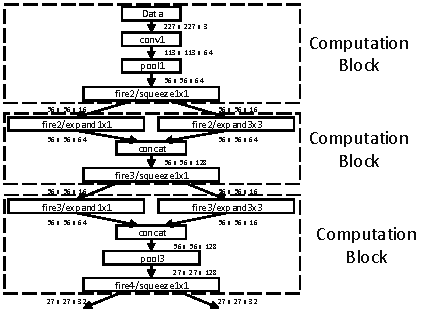
\includegraphics[width=0.35\textwidth]{squz.pdf}}
\caption{SqueezeNet sliced into computation block}
\label{sqz}
\end{figure}
\subsection{Strategy II: Computation block}
Computation block is the key feature in our design. It is a collection of layers fused together as a single block. It contains expand layers(3x3, 1x1 convolution) followed by a max pool, squeeze layer(1x1 convolution) and finally average pool layer. With all these layers computation block will easily fit into any small FPGA like cyclone V. Fig.~\ref{sqz} Show how Squeezenet is sliced into 9 partitions which can be executed in our computation block in a sequential manner without reprogramming the hardware. Here is the list of main features of computation blocks

\begin{itemize}
\item Configurable size: size of input dimension, number of kernels can be configured on the fly by setting configuration registers and computation block will operate accordingly. This make computation block can be reused for different size of input and number of the kernel within the provided range.

\item Configurable layers: layers inside computation block can be enabled or disabled through control signal or by API. This makes computation blocks to operate in a different mode. For example, at the start of SqueezeNet model, only 3x3 convolution is enabled and at the end, only 3x3 and average pool are enabled.

\item Low memory footprint: computation block won't begin with squeeze layer as in fire module of SqueezeNet. We purposely did this because, after squeeze layer, model shirks to fewer size, so slicing the model after squeeze layer and making it as entry and exit point of the computation block will reduce memory access. And the intermediate results after expand layer, which is larger in size, are processed internally without sending to memory. This cleaver decision has enormously reduced the memory bandwidth demand. 


\item Cascadable design: computation generate the out as in the same order of the input. This makes computation block cascadable. For example in a larger FPGA, we can put two computation block one after another. This will increase the throughput by more than 2 times.

\item Compact size: computation block contains few collections of layers though it is compact in size and can be accommodated small FPGA too. So computation block can be a general solution across different devices.

\end{itemize}

\section{Architecture}
\subsubsection{System architecture}

\begin{figure}[htbp]
\centerline{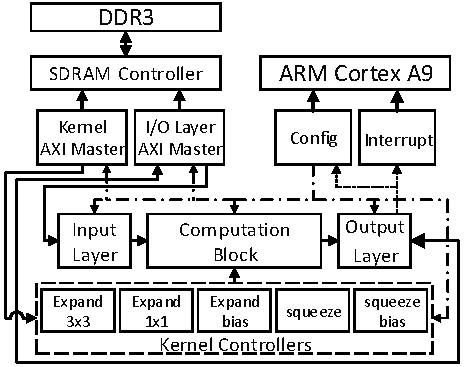
\includegraphics[width=0.36\textwidth]{archiecture.pdf}}
\caption{System architecture}
\label{arch}
\end{figure}

Fig.~\ref{arch} shows the overall architecture of our design. the host processor(\textit{ARM cortex 9}) can access the memory through SDRAM controller. It will write all model parameters and input data in a shared memory space. Final output can be read from the shared memory space. There is an AXI bus between host and FPGA(\textit{config}) to transfer configuration parameter, address spaces of data location from the host processor to FPGA. There is an interrupt signal from FPGA to denote the completed task. In hardware side, we have two AXI master connected to \textit{input layer} block and \textit{output layer} block, one is to read model parameters and another one is to read, write input and output feature map. \textit{config} module set the configuration register of all other modules, such that each module know how to operate. It sends the addresses to \textit{input layer} and \textit{kernel controller} block, which denotes the location of data. \textit{input layer} module read the input data from DDR memory and \textit{kernel controller} module read the weights, bias. once \textit{computation block} received configuration it knows which layers to enable, input dimension, number of kernels operation need to be done etc. then it sends the data to \textit{output layer} module. Output layer writes the result in DDR memory in the allocated location. When execution of the whole iteration of computation block finishes, \textit{output layer} send an interrupt to the host processor.


\subsubsection{computation block}

\begin{figure}[htbp]
\centerline{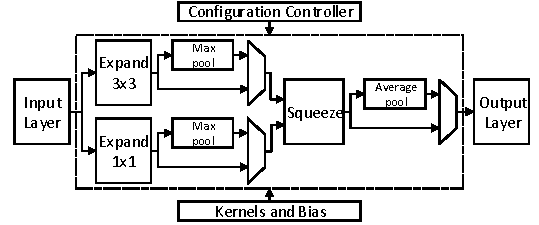
\includegraphics[width=0.4\textwidth]{computation.pdf}}
\caption{computation block architecture}
\label{cmp}
\end{figure}


Fig.~\ref{cmp} shows the architecture of the computation block and its interface with other blocks. A computation block consists of four different layers, including the two expand convolution (3x3 and 1x1), max pool layer, one squeeze layer (1x1 convolution) and an average pool layer. Expand layer has 4 parallel pipelines followed by an adder tree and RELU activation. We can enable max pool or average pool function by configuring computation block accordingly.






% \begin{table*}[t]
%   \centering
%   \begin{tabular}{*{4}{c}}
%     \hline 
% 	& CASE I 	&	CASE II 	& 	 CASE III \\
% 	\hline
% 	Input size & 56 x 56 & 56 x 56 & 56 x 56 \\
% 	\hline
% 	Input Depth & 16 & 16 & 16 \\
% 	\hline
% 	No of Kernels & 64 & 64 &  64 \\ 
% 	\hline
% 	clocks required &  56 x 56 x 16 x 64 / 4   = 802816 &  56 x 56 x 16 x 64 / 4   = 802816 & 56 x 56 x 16 x 64 / 4   = 802816 \\ 
% 	\hline
% 	Max pool & enable &  disable & disable \\
% 	\hline
% 	Squeeze size &  27 x 27 & 56 x 56 & 56 x 56 \\
% 	\hline
% 	Squeeze depth &  64 + 64 = 128 & 64 + 64 = 128 & 64 + 64 = 128 \\
% 	\hline
% 	No. Squeeze Kernels  & 16 &  32 & 48 \\
% 	\hline
% 	Squeeze Layer Computation Clocks & 27 x 27 x 128 x 16 / 16 = 93312 & 56 x 56 x 128 x 32 / 16 = 802816 & 56 x 56 x 128 x 48 / 16 = 1204224 \\
% 	\hline
% 	Time (@ 100MHz) & 8.02 ms & 8.02 ms &12.04 ms \\
% \hline
%   \end{tabular}
%   \caption{Time for computation block in three different scenario}
%   \label{tab2}
% \end{table*}


\section{Implementation}
%\subsubsection{Functional flow}

First, we have to train the CNN model using TensorFlow or any framework. It's better to use SqueezeNet like models will achieve the highest efficiency in our architecture. Then select appropriate floating point representation required for the trained model by empirical experiment. Then convert trained weights and bias parameters to custom floating point values using provided APIs. This initial part can be done offshore in servers. Now converted parameters handed over to ARM processor in SoC FPGA. A host program also compiled and loaded in processor. Host program loads the parameter in memory and sends the address to FPGA, so it can access parameters. Then host program generates the configuration parameters required to execute a particular CNN model and send it to the \textit{config} module in FPGA. After initializing, it will start to load the input images into memory and pass the address to FPGA. 
In FPGA, the configuration controller reads configurations and distributes to all other modules (\textit{input layer, an output layer, kernel loader, computation block}). Eventually, it will set all the required configuration registers in these modules. configuration controller issue a \textit{start} signal to all blocks. Now weights and input data are read from memory and fed to kernel controller and input layer modules. They will rearrange the order as required by computation block. Then computation block processes the data according to configurations. The output from the computation block sends to output layer module which will write the output to memory. Again in next iteration input are read from memory and configuration block is executed with another configuration. This loop continues until it reaches the final layer. After the final iteration, the configuration controller generates an interrupt to host programme denoting that inference have completed. Now host program can access the output of inference and use it to perform the higher level task. Copying the next input image can be done parallelly while computation on the previous image by using an interrupt signal. So we can continuously execute inference like a real-time system without any delay for setting up input image.


\section{Experimental results}\label{SCM}


Experiments were conducted in DE 10 Nano board. We have used trained weights from \cite{weight} and converted them to 8-bit float and loaded the model. Using custom floating point number only reduced 6\% of the accuracy hence our architecture achieved around 51\% top 1 accuracy in Imagenet dataset. It took around 110ms for executing all computation blocks, hence our architecture achieved around 9FPS which is more than enough in most of the embedded vision application.

Table.~\ref{tab2} show the measured performance of three different cases. Expand convolutions and squeeze convolution execute simultaniously. In first two case expand decided the execution time of computation block in the last case squeeze decide the execution time. Case I,II show that enabling maxpool (for average pool too) will not affect the execution time.


\begin{table}[htbp]
\caption{Time for computation block in three different scenario}
\begin{tabular}{|l|l|c|c|c|}
\hline
\multicolumn{2}{|l|}{Layers}               & \multicolumn{1}{l|}{Case I}  & Case II & Case III \\ \hline
\multirow{4}{*}{Expand}  & Input size      & 56 x 56                      & 56 x 56 & 56 x 56  \\ \cline{2-5} 
                         & Input Depth     & 16                           & 16      & 16       \\ \cline{2-5} 
                         & No of Kernels   & 64                           & 64      & 64       \\ \cline{2-5} 
                         & clocks required & 802,816                      & 802,816 & 802,816  \\ \hline
\multicolumn{2}{|l|}{Max pool}             & \multicolumn{1}{l|}{enable}  & disable & disable  \\ \hline
\multirow{4}{*}{squeeze} & size            & 27 x 27                      & 56 x 56 & 56 x 56  \\ \cline{2-5} 
                         & depth           & 128                          & 128     & 128      \\ \cline{2-5} 
                         & No of kernels   & 16                           & 32      & 48       \\ \cline{2-5} 
                         & clock required  & 93,312                       & 802,816 & 1204,224 \\ \hline
\multicolumn{2}{|l|}{Total time @ 100MHz}  & \multicolumn{1}{l|}{8.02 ms} & 8.02 ms & 12.04 ms \\ \hline
\end{tabular}
  \label{tab2}
\end{table}


\begin{table}[]
\caption{Memory access of computation block when implementing SqueezeNet}
\begin{tabular}{|c|c|c|c|c|}
\hline
No    & Input KB    & Weights KB    & Output KB   & Total KB \\ \hline
1     & 463.761     & 197.504       & 50.176      & 557      \\ \hline
2     & 150.528     & 519.168       & 50.176      & 670      \\ \hline
3     & 150.528     & 521.216       & 23.328      & 530      \\ \hline
4     & 69.984      & 1007.616      & 23.328      & 1078     \\ \hline
5     & 69.984      & 1011.712      & 8.112       & 1066     \\ \hline
6     & 24.336      & 1105.92       & 8.112       & 1130     \\ \hline
7     & 24.336      & 1112.064      & 10.816      & 1140     \\ \hline
8     & 32.448      & 1966.08       & 10.816      & 2000     \\ \hline
9     & 32.448      & 8589.312      & 1           & 8612     \\ \hline
\multicolumn{4}{|l|}{Total Memory to be accessed} & 1700     \\ \hline
\multicolumn{5}{|l|}{Required Bandwidth for 9FPS = 142MB/s}  \\ \hline
\end{tabular}
\label{tab3}
\end{table}


Table.\ref{tab3} Show the memory usage in each iteration of the computation block. Calculated average bandwidth for our architecture is around 142MB/s. It also shows that the final convolution layer which performs the classification requires the highest bandwidth

% 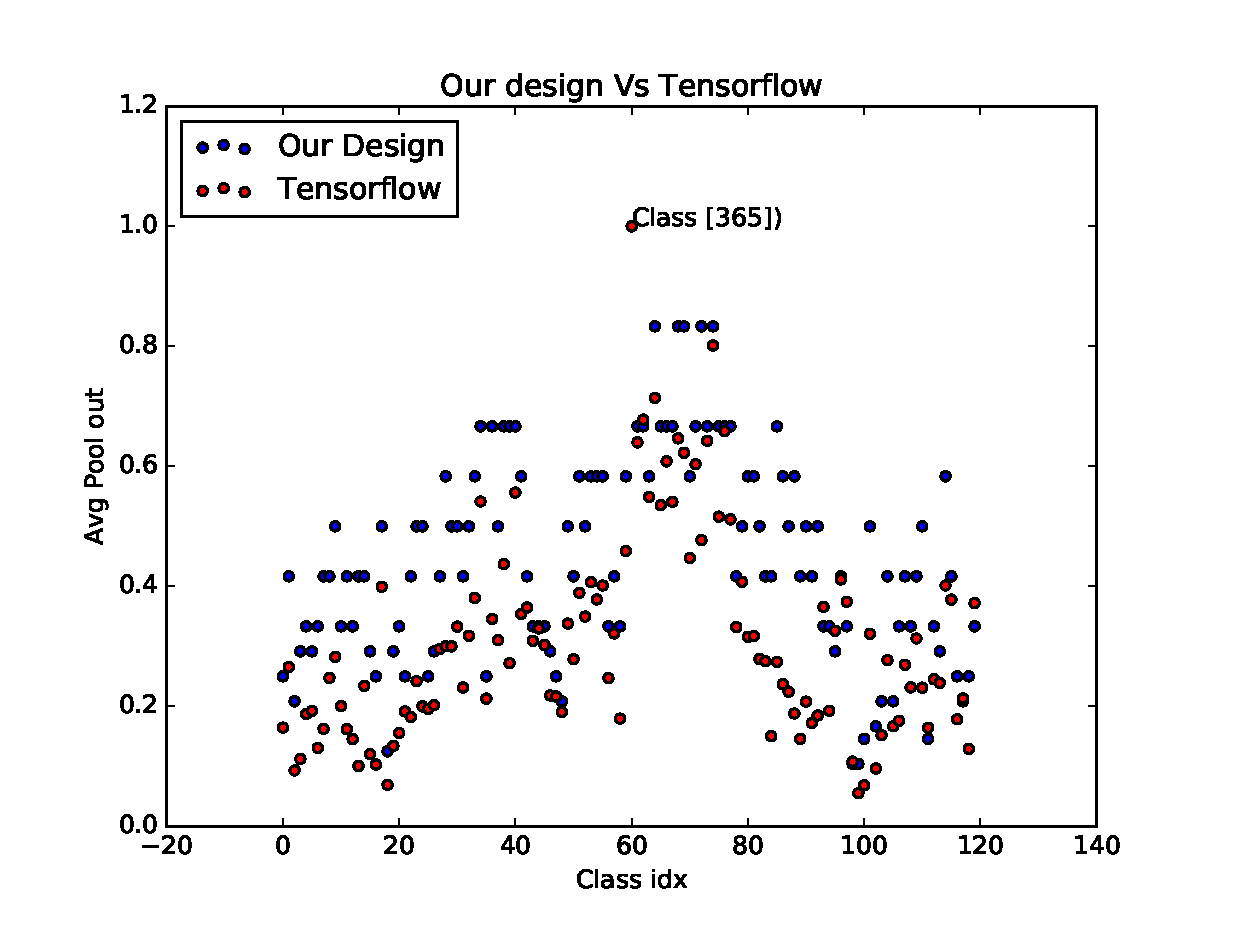
\epsfig{file=plot.eps,width=1\linewidth}

\begin{figure} 
   \centering
 % \subfloat[]{%
 %      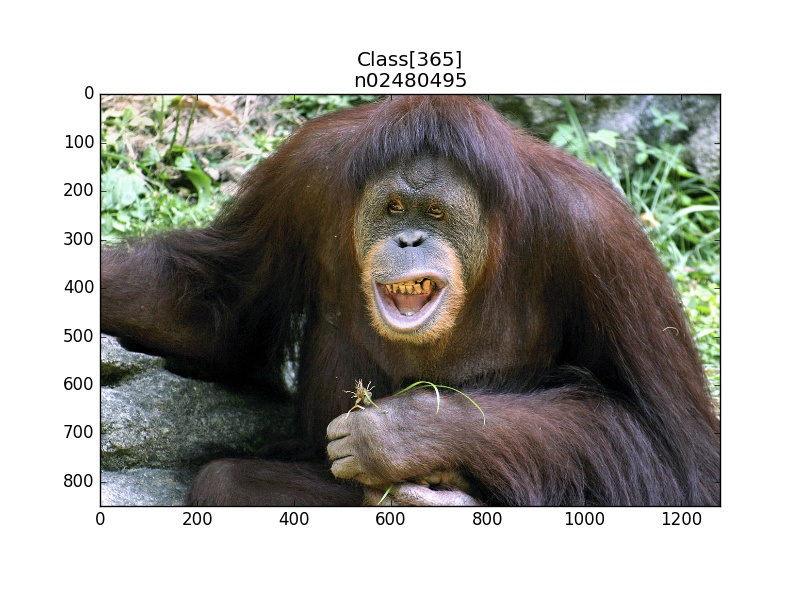
\includegraphics[width=0.28\linewidth,valign=c]{image.jpg}}
 %   \label{1a}
 \subfloat[]{%
       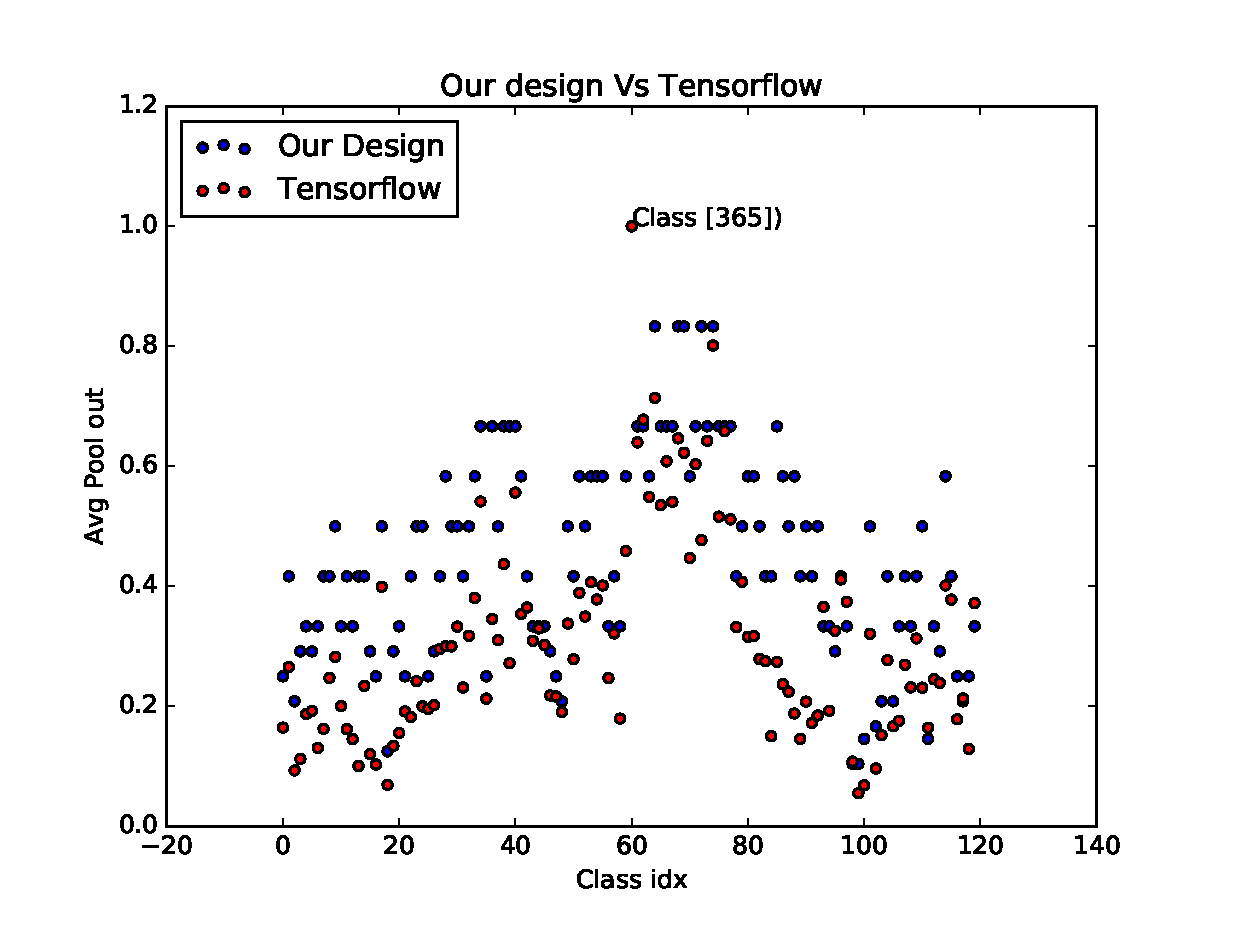
\includegraphics[width=1\linewidth,valign=c]{plot.eps}}
   \label{1b}
 \caption{comparision of class score from our design and 32-bit implementation for a sample image}
 \label{fig1} 
\end{figure}


Fig. ~\ref{fig1} show the final value for a sample image from 32 bit (TensorFlow) and from our design. We can see quantization error due to custom float representation. Still, it have correctly predicted the class. 



\section{Discussion}
In our study we quantize pretrained network to 8 bit floating numbers, which may affect the accuracy due to quantization error. Improvement can be done by retraining the model starting from pretrained quantized parameters. By retraining model will adjust to quantization error and adapts to custom number system, this may improve the accuracy.

\section*{Acknowledgment}
The authors would like to thank InnovateFPGA community for valueable feedback.

\bibliographystyle{IEEEtran}
\bibliography{IEEEabrv,mybibfile}


\end{document}
